\documentclass{amsart}
\usepackage{tikz}
\usepackage{float}

\usepackage{amsmath}
\usepackage{amsfonts}
\usepackage{amsthm}
\usepackage{enumitem}
\usepackage{dsfont}
\usepackage{amssymb}
\usepackage{pifont}
\usepackage{mathtools}

\newtheorem{thm}{Theorem}[section]
\newtheorem{lem}[thm]{Lemma}
\newtheorem{prop}[thm]{Proposition}
\newtheorem{conj}[thm]{Conjecture}
\newtheorem{cor}[thm]{Corollary}

\newtheorem*{prop*}{Proposition}

\theoremstyle{definition}
\newtheorem{claim}[thm]{Claim}
\newtheorem{defn}[thm]{Definition}
\newtheorem{quest}[thm]{Question}
\newtheorem{remark}[thm]{Remark}
\newtheorem{fact}[thm]{Fact}
\newtheorem{note}[thm]{Note}

\newtheorem*{claim*}{Claim}
\newtheorem*{quest*}{Question}
\newtheorem*{remark*}{Remark}
\newtheorem*{fact*}{Fact}

\newcommand{\N}{\ensuremath{\mathbb{N}}}
\newcommand{\Z}{\ensuremath{\mathbb{Z}}}
\newcommand{\Q}{\ensuremath{\mathbb{Q}}}
\newcommand{\R}{\ensuremath{\mathbb{R}}}
\newcommand{\C}{\ensuremath{\mathbb{C}}}
\newcommand{\F}{\ensuremath{\mathbb{F}}}
\newcommand{\AP}{\ensuremath{\mathcal{A}_{2^{n}}}}
\newcommand{\BP}{\ensuremath{\mathcal{B}_{2^{n}}}}
\newcommand{\CP}{\ensuremath{\mathcal{C}_{2^{n}}}}
\newcommand{\DP}{\ensuremath{\mathcal{D}_{2^{n}}}}
\newcommand{\EP}{\ensuremath{\mathcal{E}_{2^{n}}}}
\newcommand{\FP}{\ensuremath{\mathcal{F}_{2^{n}}}}

\newcommand{\E}{\ensuremath{\mathbb{E}}}
\newcommand{\1}{\ensuremath{\mathds{1}}}

\newcommand{\pair}[2]{\ensuremath{\langle #1, #2 \rangle}}

\DeclareMathOperator{\Gal}{Gal}
\DeclareMathOperator{\Jac}{Jac}
\DeclareMathOperator{\Var}{Var}
\DeclareMathOperator{\Cov}{Cov}
\DeclareMathOperator{\Div}{Div}
\DeclareMathOperator{\Prin}{Prin}        
\DeclareMathOperator{\im}{im}
\DeclareMathOperator{\val}{val}

\newcommand{\bv}[1]{\widehat{\mathbf{#1}}}
\renewcommand{\thefootnote}{\fnsymbol{footnote}}

\title{Jacobians of finite graphs and the monodromy pairing}
\author{Louis Gaudet, Nicholas Wawrykow, Theodore Weisman}

\begin{document}

\maketitle

Unless stated otherwise, we will take a ``graph'' to mean a finite
connected multigraph with no loops.

\section{Jacobians of Finite Graphs}
\label{sec:jacobians}

\subsection{The general graph case}
It is natural to ask which finite abelian groups appear as Jacobians
of graphs. The problem can be considerably reduced by the following
proposition:

\begin{prop}
\label{prop:wedge_product}
Let $G_1$ and $G_2$ be graphs. Then $\Jac(G_1 \vee G_2) \simeq
\Jac(G_1) \times \Jac(G_2)$.
\end{prop}

We prove Proposition \ref{prop:wedge_product} by observing that the
Jacobian of a graph can be directly computed from the Smith normal
form of its Laplacian matrix. Throughout the following, for any
integer matrix $M$, let $M_{i,i}$ represent the submatrix of $M$ obtained
by deleting the $i$th row and column.

\begin{lem}
\label{lem:SNF_submatrix}
Let $G$ be a graph, and let $Q$ be the Laplacian matrix of $G$. If the
Smith normal form of $Q$ is $S$, then for any $i$, the Smith normal
form of $Q_{i,i}$ is $S_{n,n}$.
\end{lem}
\begin{proof}
  WE NEED A PROOF OF THIS, but I feel like someone has to have proved
  it already so I'm not typing it.
\end{proof}

\begin{proof}[Proof of Proposition \ref{prop:wedge_product}]
  Let $Q_1$ and $Q_2$ be the Laplacian matrices of $G_1$ and $G_2$,
  respectively, and let the vertex of intersection of $G_1$ and $G_2$
  be $v_0$. Enumerate the vertices of $G$ so that the Laplacian of $G$
  can be written as
\begin{equation*}
  Q = 
  \left[\begin{array}{ccc}
      Q_1 & \vdots & \\
      \ldots & \val{v_0}  & \ldots \\
      & \vdots & Q_2
  \end{array}\right]
\end{equation*}
If we delete the row and column corresponding to $v_0$, the resulting
matrix $Q'$ will be in block diagonal form, and has cokernel
isomorphic to that of the matrix obtained by taking the Smith normal
form of the blocks. Applying Lemma \ref{lem:SNF_submatrix}, we then
see that the following matrix $M$ has cokernel isomorphic to the
cokernel of $Q$:

\begin{equation*}
  \left[\begin{array}{cc|c}
      S_1 & \\
      & S_2 \\ \hline
      & & 0
    \end{array}\right]
\end{equation*}

where $S_1$, $S_2$ are diagonal matrices whose entries are the
invariant factors of $\Jac(G_1), \Jac(G_2)$, respectively.
\end{proof}

\begin{figure}[h]
  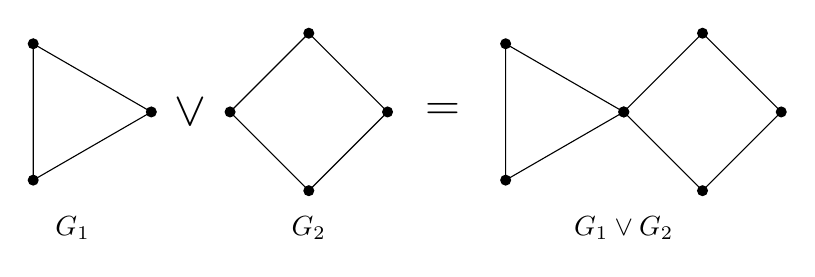
\begin{tikzpicture}    
    \draw {(0:1) -- (120:1) -- (240:1)} -- cycle (270:1.2) node[below]
    {$G_1$};
    \foreach \theta in {0, 120, 240} {
      \fill (\theta:1) circle (2pt) ;
    } ;

    \node at (0:1.5) {\LARGE $\vee$};

    \begin{scope}[xshift=3cm]
      \draw {(0:1) -- (90:1) -- (180:1) -- (270:1)} -- cycle (270:1.2)
      node[below] {$G_2$};

      \foreach \theta in {0, 90, ...,  270} {
        \fill (\theta:1) circle (2pt) ;
      } ;
    \end{scope}

    \node at (0:4.7) {\LARGE $=$} ;

    \begin{scope}[xshift=6cm]
      \draw {(0:1) -- (120:1) -- (240:1)} -- cycle ;
      \foreach \theta in {0, 120, 240} {
        \fill (\theta:1) circle (2pt) ;
      } ;
      \begin{scope}[xshift=2cm]
        \draw {(0:1) -- (90:1) -- (180:1) -- (270:1)} -- cycle ;
        
        \foreach \theta in {0, 90, ...,  270} {
          \fill (\theta:1) circle (2pt) ;
        } ;
      \end{scope}
      \node[below] at (1,-1.2) {$G_1 \vee G_2$} ;
    \end{scope}
  \end{tikzpicture}
  \caption{The wedge sum operation on graphs. In this case, $\Jac(G_1)
  \simeq \Z/3\Z$, $\Jac(G_2) \simeq \Z/4\Z$, and $\Jac(G_1 \vee G_2)
  \simeq \Z/12\Z$.}
\end{figure}

Note that in the case that $G_1$ is a tree (and therefore $\Jac(G_1)$
is trivial), $\Jac(G_1 \vee G_2) \simeq \Jac(G_2)$. We then have
the following corollary:
\begin{cor}
  \label{cor:1_valent}
  Let $G$ be a graph, and let $A = \{v \in V(G) : \val(v) > 1\}$. If
  $G'$ is the subgraph of $G$ induced by $A$, then $\Jac(G) \simeq
  \Jac(G')$.
\end{cor}

Proposition \ref{prop:wedge_product}, together with the classification
theorem for finite abelian groups, tells us that if, for all $n$,
there exists a graph $G$ such that $\Jac(G)$ is cyclic of order $n$,
then \emph{all} finite abelian groups are the Jacobian of some graph.

For given $n$, we give two possible constructions of $G$ with $\Jac(G)
\simeq \Z/n\Z$.

\begin{defn}
  $B_n$, the \emph{banana graph on $n$ edges}, is the graph with
  $V(B_n) = \{v_1, v_2\}$ and edge multiset consisting of $n$ copies of
  $\{v_1, v_2\}$.
\end{defn}

\begin{figure}[h]
  \begin{center}
    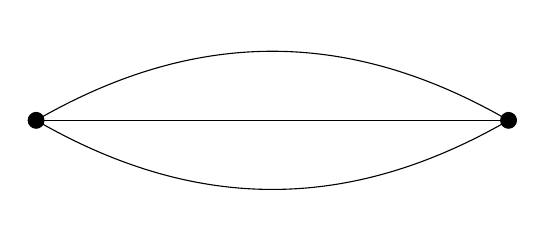
\begin{tikzpicture}
      \draw (0,0) to [out=30, in=150] (6,0) ;
      \draw (0,0) to [out=-30, in=-150] (6,0) ;
      \draw (0,0) to [out=0, in=180] (6,0) ;

      \draw [fill] (0,0) circle [radius=.1cm] ;
      \draw [fill] (6,0) circle [radius=.1cm] ;      
    \end{tikzpicture}
    \caption{The $3$-banana $B_3$}
  \end{center}
\end{figure}

\begin{prop}
  \label{prop:banana_cyclic}
  Let $B_n$ be the banana graph on $n$ edges. Then $\Jac(B_n) \simeq \Z/n\Z$.
\end{prop}

\begin{proof}
  $B_n$ has $n$ spanning trees, so
  $|\Jac(B_n)| = n$. To show that $\Jac(B_n) \simeq \Z/n\Z$, it
  suffices to find a single element of order at least $n$.

  Let $D \in \Div^0(B_n)$ be the divisor $(v_2) - (v_1)$, and consider
  $\overline{D} = \in \Jac(B_n)$. For any $1 \le m < n$, the divisor
  $mD$ is $v_1$-reduced---since $v_2$ has degree $n$, it is impossible
  to fire it without sending it into debt. If $m=n$, then firing $v_2$
  yields the zero divisor. $m\overline{D}$ is therefore trivial iff
  $m$ is a multiple of $n$, and hence $\overline{D}$ has order $n$ as
  required.
\end{proof}

\subsection{The simple graph case}
The construction given above is sufficient to show that all finite
abelian groups appear as the Jacobian of some graph. However, since
banana graphs are only realizable as a multigraphs, it is natural to
ask whether there also exists a family of simple graphs $G$ such that
$\Jac(G) \simeq \Z/n\Z$ for given $n$. Below, we provide such a
construction for all $n > 2$. 

\begin{lem}
  \label{lem:2valent_path}
  Let $G$ be a graph, and suppose that for some path $P$ with vertices
  $\{v_1, \ldots, v_\ell\}$ on $G$, $\val(v_i) = 2$ for all $1 < i <
  \ell$. If $D$ is the divisor $(v_2) - (v_1)$, then, for any $1 < m <
  \ell$,
  \begin{equation*}
    mD \sim (v_{m+1}) - (v_1)
  \end{equation*}
\end{lem}
\begin{proof}
  Under an appropriate enumeration of the vertices of $G$, the
  Laplacian matrix $Q$ of $G$ has the form

  $$Q = \begin{bmatrix}
    k_1 & -1 \\
    -1 &  2 & -1 \\
    & -1 &  2 & -1 \\
    &    &    &  \ddots  \\
    &    &    &  -1 & k_\ell \\ 
    &    &    &     &    & \ddots
  \end{bmatrix}$$

  where $k_1$ and $k_\ell$ are the degrees of $v_1$ and $v_\ell$,
  respectively. Since the equivalence relation on divisors is defined
  by the image of the Laplacian map $\Delta$, the claim is equivalent
  to the statement that there exists $\mathbf{v} \in \Z^n$ such that

  \begin{equation*}
    \bv{v}_{m+1} - \bv{v}_1  = m(\bv{v}_2 - \bv{v}_1) + Q\mathbf{v}
  \end{equation*}

  where $\bv{v}_i$ represents the $i$th standard basis element for
  $\Z^n$, corresponding to the divisor with formal sum $(v_i)$. If we
  choose $\mathbf{v} = \sum_{i=1}^{m - 1}(m - i)\bv{v}_i$, it is
  easy to check that the equality above holds.
\end{proof}

\begin{cor}
  \label{cor:2valent_path}
  Let $G$ be any biconnected graph that contains a path $P$ as
  above. Then $\Jac(G)$ contains an element of order at least $\ell$.
\end{cor}
\begin{proof}
  Let $m < \ell$, and consider $D = (v_2) - (v_1)$. $G$ is
  biconnected, so there is a path from $v_1$ to $v_{m+1}$ that does
  not contain any vertex $v_i$ for $1 < i < m$. Applying the burning
  algorithm then shows that the divisor $(v_{m+1}) - (v_1)$ is
  $v_1$-reduced, and hence $m\overline{D}$ is nonzero for $m < \ell$,
  as required.
\end{proof}

\begin{cor}
  \label{prop:cycle_cyclic}
  Let $C_n$ be the cycle graph on $n \ge 2$ vertices. Then $\Jac(C_n) \simeq
  \Z/n\Z$.
\end{cor}
\begin{proof}
$C_n$ has $n$ spanning trees, so $|\Jac(C_n)|=n$ and, as before, it
suffices to find a single element of $\Jac(C_n)$ of order at least
$n$. Corollary \ref{cor:2valent_path} guarantees that such an element
exists.
\end{proof}

$C_n$ is a simple graph whenever $n > 2$, so we have the following

\begin{cor}
  Let $\Gamma$ be a finite abelian group that is not isomorphic to
  $\Z/2\Z \times H$ for any group $H$. Then there exists a simple
  graph $G$ such that $\Gamma \simeq \Jac(G)$.
\end{cor}

The rest of this section will investigate which groups $\Gamma =
\Z/2\Z \times H$ can possibly occur as the Jacobian of some simple
graph. It is known that there is no simple graph $G$ with $\Jac(G)
\simeq \Z/2\Z$, since there is no simple graph with two spanning
trees. 

We will generalize this result, first examining the case that the
graph $G$ is biconnected. We motivate this restriction by noting that
there is a sense in which biconnected graphs generate all other
graphs: when $G$ is not biconnected, then by definition, there is a
vertex $v_0$ such that the subgraph $G'$ induced by $V(G) \setminus
\{v_0\}$ is not connected. $G$ is then the wedge sum of the connected
components of $G'$ (together with the vertex $v_0$), and so $\Jac(G)$
splits as a direct product of Jacobians of subgraphs of $G$.

\begin{defn}
  Let $G$ be a graph, and let $\Gamma = \Jac(G)$. We will write $\mu(G)$
  for the maximum order of an element of $\Gamma$, and $\delta(G)$ for
  the maximum valency of a vertex in $G$. (When the graph $G$ is clear
  from context, we will simply write $\delta$ or $\mu$). 
\end{defn}

\begin{lem}
  \label{lem:delta_le_mu}
  If $G$ is biconnected, then $\delta(G) \le \mu(G)$. Furthermore, if
  $\delta(G) = \mu(G)$, then $G$ must be the banana graph $B_\mu$.
\end{lem}
\begin{proof}
  Let $v$ be a vertex in $V(G)$ with valency $\delta$, and let $w$ be
  a vertex adjacent to $v$. Consider the divisor $D = (v) -
  (w)$, and let $m < \delta$ be a positive integer. 

  We apply Dhar's burning algorithm to check that $mD$ is
  $w$-reduced. Since $G$ is biconnected, there is a path from $w$ to
  each of the neighbors of $v$ that does not contain $v$, and so each
  of the neighbors of $v$ is burned during the algorithm. $v$ has more
  than $m$ distinct neighbors, so it is burned as well. Therefore,
  $m\overline{D}$ is nonzero and $\overline{D}$ has order at least
  $\delta$.

  In the case that $\delta = \mu$, we must have $\delta\overline{D} =
  0$. Starting from $\delta D$, chip-fire $v$ once, and let the divisor
  we obtain be $E$. Applying the burning algorithm and the
  biconnectivity condition once more, we see that $v$, as well as each
  of its neighbors, must be burned, and therefore that $E$ is
  zero. This is only possible if the multiplicity of the edge
  $\{v,w\}$ is $\delta$, i.e. $G$ is a banana graph.
\end{proof}

\begin{cor}
  \label{cor:genus_v_mu}
  For any biconnected graph with genus $g$ and $|V(G)| = n$,
  \begin{equation*}
    n \ge \frac{2g - 2}{\mu - 1}.
  \end{equation*}
\end{cor}
\begin{proof}
  Let $e = |E(G)|$. We have 
  \begin{equation*}
    2e = \sum_{i=1}^n \val(v_i) \le \sum_{i=1}^n \delta = n \cdot \delta
    \le n \cdot \mu.
  \end{equation*}
  Since $e = g + n - 1$, this gives $2g - 2 \le n \cdot (\mu - 1)$, as
  required.
\end{proof}

We now prove the first of our main results:

\begin{thm}
  \label{thm:2group}
  For any $k \ge 1$, if $G$ is a graph such that $\Jac(G) \simeq
  (\Z/2\Z)^k$, then $G$ is not simple.
\end{thm}

\begin{proof}[Proof of Theorem \ref{thm:2group}]
  Let $G$ be a biconnected graph with $\Jac(G) = (\Z/2\Z)^k$. By
  Corollary \ref{cor:1_valent}, we may assume without loss of
  generality that each vertex of $G$ has valency at least $2$. By
  Lemma \ref{lem:delta_le_mu}, each vertex of $G$ has valency exactly
  $2$, hence $G = C_n$ for some $n$. We must have $n=2$, which means $G$
  cannot be simple.

  Now let $G$ be a graph that is not biconnected, with $\Jac(G) \simeq
  (\Z/2\Z)^k$. We proceed by induction on $k$.
  
  The base case $k=1$ is known. For $k > 1$, note that $\Jac(G) \simeq
  \Jac(G_1) \times \Jac(G_2)$ for connected subgraphs $G_1, G_2$ of
  $G$. Without loss of generality, $G_2$ is not a tree, and hence
  $\Jac(G_1) \simeq (\Z/2\Z)^{k_1}$ for $k_1 < k$. By the inductive
  hypothesis, $G_1$ is not simple, and so neither is $G$.
\end{proof}

\begin{remark}
  The proof of Theorem \ref{thm:2group} also gives a complete
  characterization of any graph $G$ with $\Jac(G) \simeq
  (\Z/2\Z)^k$. In general, we can always obtain $G$ from the following
  construction: starting with some tree $T$, choose $k$ edges of $T$,
  and give those edges multiplicity $2$. We will apply this
  characterization later, in our discussion of the monodromy pairing
  on $\Jac(G)$.
\end{remark}

\begin{figure}[H]
  \begin{center}
    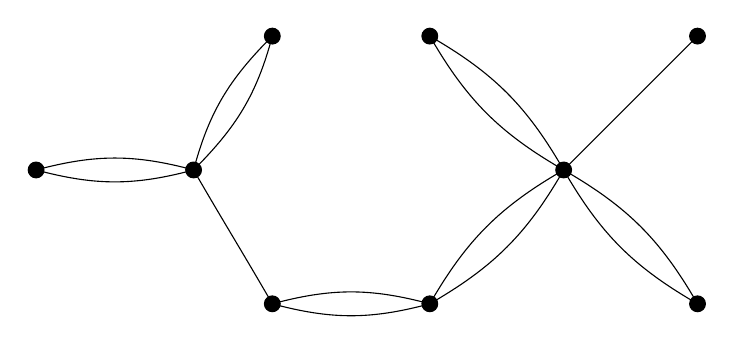
\begin{tikzpicture}

      \draw (0,0) to [out=15, in=165] (2,0) ;
      \draw (0,0) to [out=-15, in=-165] (2,0) ;

      \draw (2,0) to [out=75, in=225] (3, 1.7) ;
      \draw (2,0) to [out=45, in=255] (3, 1.7) ;

      \draw (2,0) to [out=-60, in=-240] (3, -1.7) ;

      \draw (3,-1.7) to [out=15, in=165] (5, -1.7) ;
      \draw (3,-1.7) to [out=-15, in=-165] (5, -1.7) ;

      \draw (5, -1.7) [out=60, in=210] to (6.7, 0) ;
      \draw (5, -1.7) [out=30, in=240] to (6.7, 0) ;

      \draw (6.7, 0) [out=120, in=-30] to (5, 1.7) ;
      \draw (6.7, 0) [out=150, in=-60] to (5, 1.7) ;

      \draw (6.7, 0) to (8.4, 1.7) ;

      \draw (6.7, 0) to [out=-30, in=120] (8.4, -1.7) ;
      \draw (6.7, 0) to [out=-60, in=150] (8.4, -1.7) ;

      \draw [fill] (0,0) circle [radius=.1cm] ;
      \draw [fill] (2,0) circle [radius=.1cm] ;
      \draw [fill] (3,1.7) circle [radius=.1cm] ;
      \draw [fill] (3,-1.7) circle [radius=.1cm] ;
      \draw [fill] (5,-1.7) circle [radius=.1cm] ;
      \draw [fill] (6.7, 0) circle [radius=.1cm] ;
      \draw [fill] (5,1.7) circle [radius=.1cm] ;
      \draw [fill] (8.4,1.7) circle [radius=.1cm] ;
      \draw [fill] (8.4,-1.7) circle [radius=.1cm] ;
    \end{tikzpicture}
    \caption{An example of a graph $G$ with $\Jac(G) \simeq
      (\Z/2\Z)^6$}
  \end{center}
\end{figure}

We will now generalize this result to graphs whose Jacobian is of the
form $(\Z/2\Z)^k \times H$, using a similar inductive argument on
biconnected subgraphs. Throughout the following, we will suppose that
$G$ is a biconnected graph with Jacobian $\Jac(G) = \Gamma \simeq
(\Z/2\Z)^k \times H$ for some finite abelian group $H$, and that $\mu$
is the maximum order of an element of $H$. We will require the
following bound on the genus of $G$:

\begin{thm}[CITE LORENZINI]
  \label{lem:genus_cycle}
  If $g$ is the genus of $G$, then $g \ge k$.
\end{thm}

Applying Corollary \ref{cor:genus_v_mu} to this result shows that 
\begin{equation*}
  |V(G)| \ge \frac{2k-2}{\mu - 1}
\end{equation*}
We now establish an upper bound on $|V(G)|$ in terms of $\mu$ and
$|H|$, to achieve an upper bound on $k$.

\begin{prop}
  \label{prop:v_bound}
  Suppose that $G$ is biconnected. Then for any finite abelian group
  $H$, there exists an integer $v_0$ (depending only on $H$) such that
  if $\Gamma = \Jac(G) \simeq (\Z/2\Z)^k \times H$, then $|V(G)| <
  v_0$.
\end{prop}

\begin{proof}
  Let $U = \{u \in V(G) : \val(u) > 2\}$, and enumerate the elements
  of $U$ as $u_1, \ldots, u_m$. We will first establish a bound on
  $m = |U|$, and then bound $|V(G)|$ in terms of $m$.
  
  Consider the set of divisors $\mathcal{U} = \{(u_i) - (u_1) : 1 \le
  i \le m\}$, and let $\overline{\mathcal{U}} \subseteq \Gamma$ be the
  set of equivalence classes of the elements of $\mathcal{U}$. Write
  $D_i$ for $(u_i) - (u_1)$. For any $D_i, D_j \in \mathcal{U}$, we
  claim that $2D_j - 2D_i$ is $u_i$-reduced.

  We have $2D_j - 2D_i = 2(u_j) - 2(u_i)$. Since $G$ is biconnected,
  there is a path from $u_i$ to each of the neighbors of $u_j$ that
  does not contain $u_j$. Since $u_j$ has valency at least $3$, an
  iteration of the burning algorithm must burn $u_j$, and in turn the
  entire graph. Furthermore, since $2D_j - 2D_i$ is $u_i$-reduced,
  $2\overline{D_j} \ne 2\overline{D_i}$ for any $i \ne j$. Note that
  this also implies that $\overline{D_j} \ne \overline{D_i}$ for any
  $i \ne j$, so we have $m=|\overline{\mathcal{U}}|$.

  We now define a map
  \begin{align*}
    \phi: \Gamma \to \Gamma \\
    \overline{D} \mapsto 2\overline{D}
  \end{align*}

  By the above, we have
  $|\phi(\overline{\mathcal{U}})|=|\overline{\mathcal{U}}|=m$. Furthermore,
  $|\im(\phi)| \le |H|$, and so we find
  $m=|\phi(\overline{\mathcal{U}})| \le |H|$ as desired.

  We now wish to bound $|V(G)|$ in terms of $m$. To do so, consider a
  graph $G'$, given by the following transformation of $G$:

  \begin{enumerate}
  \item Choose any vertex of $G$ of valency $2$. Delete it, and draw
    an edge between its neighbors.
  \item Repeat until there are no 2-valent vertices remaining.
  \end{enumerate}

  \begin{figure}[H]
    \begin{center}
      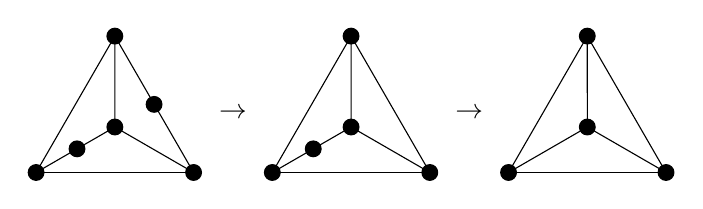
\begin{tikzpicture}

        \draw (0:0) to (60:2) ;
        \draw (0:0) to (0:2) ;
        \draw (60:2) to (0:2) ;
        \draw (0:0) to (30:1.155) ;
        \draw (0:2) to (30:1.155) ;
        \draw (60:2) to (30:1.155) ;

        \draw [fill] (0:0) circle [radius=.1cm] ;
        \draw [fill] (0:2) circle [radius=.1cm] ;
        \draw [fill] (60:2) circle [radius=.1cm] ;
        \draw [fill] (30:1.155) circle [radius=.1cm] ;
        \draw [fill] (30:.6) circle [radius=.1cm] ;
        \draw [fill] (30:1.73) circle [radius=.1cm] ;

        \draw [shift={(3,0)}] (0:0) to (60:2) ;
        \draw [shift={(3,0)}] (0:0) to (0:2) ;
        \draw [shift={(3,0)}] (60:2) to (0:2) ;
        \draw [shift={(3,0)}] (0:0) to (30:1.155) ;
        \draw [shift={(3,0)}] (0:2) to (30:1.155) ;
        \draw [shift={(3,0)}] (60:2) to (30:1.155) ;

        \draw [shift={(3,0)}][fill] (0:0) circle [radius=.1cm] ;
        \draw [shift={(3,0)}][fill] (0:2) circle [radius=.1cm] ;
        \draw [shift={(3,0)}][fill] (60:2) circle [radius=.1cm] ;
        \draw [shift={(3,0)}][fill] (30:1.155) circle [radius=.1cm] ;
        \draw [shift={(3,0)}][fill] (30:.6) circle [radius=.1cm] ;

        \draw [shift={(6,0)}] (0:0) to (60:2) ;
        \draw [shift={(6,0)}](0:0) to (0:2) ;
        \draw [shift={(6,0)}](60:2) to (0:2) ;
        \draw [shift={(6,0)}](0:0) to (30:1.155) ;
        \draw [shift={(6,0)}](0:2) to (30:1.155) ;
        \draw [shift={(6,0)}](60:2) to (30:1.155) ;

        \draw [shift={(6,0)}][fill] (0:0) circle [radius=.1cm] ;
        \draw [shift={(6,0)}][fill] (0:2) circle [radius=.1cm] ;
        \draw [shift={(6,0)}][fill] (60:2) circle [radius=.1cm] ;
        \draw [shift={(6,0)}][fill] (30:1.155) circle [radius=.1cm] ;

        \node at (2.5, .75) {$\rightarrow$} ;
        \node at (5.5, .75) {$\rightarrow$} ;

      \end{tikzpicture}
      \caption{The transformation $G \mapsto G'$}
    \end{center}
  \end{figure}

  Note that even if $G$ is simple, $G'$ need not be. It is clear,
  however, that $G$ and $G'$ have the same number of vertices with
  valency greater than $2$, and that $\delta(G) = \delta(G')$.

  By Lemma \ref{lem:delta_le_mu}, we must have that $e' = |E(G')|$ is
  at most $m \cdot \mu$ (since otherwise there would necessarily be a
  vertex of $G$ with valency greater than $\delta$). Each 2-valent
  vertex of $G$ is uniquely associated with some edge of $G'$. If
  there are more than $e' \cdot \mu$ 2-valent vertices in $G$, then at
  least $\mu$ of them are associated with a single edge of $G'$.

  In this case, $G$ would contain a path $P$ of length greater than
  $\mu$, where each vertex of $P$ has valency $2$. This would
  contradict Corollary \ref{cor:2valent_path}, so instead we have
  \[
  |V(G)| - m < m\mu^2.
  \] 
  Choosing $v_0 = |H|(1 + \mu^2)$ then gives $|V(G)| < v_0$, as
  required.
\end{proof}

Applying Corollary \ref{cor:genus_v_mu} and Lemma
\ref{lem:genus_cycle}, we see that for sufficiently large $k$, we must
have $|V(G)| > v_0$. This in turn implies that for sufficiently large
$k$, $(\Z/2\Z)^k \times H$ is not the Jacobian of any biconnected
graph.

We now complete the proof of Theorem \ref{thm:2group_product} via
induction on $|H|$.

\begin{thm}
  \label{thm:2group_product}
  Let $H$ be a finite abelian group. There exists an integer $k_0$
  (depending only on $H$) such that for all $k > k_0$, there does not exist
  a simple graph $G$ with $\Jac(G) \simeq (\Z/2\Z)^k \times H$.
\end{thm}
  
\begin{proof}[Proof of Theorem \ref{thm:2group_product}]
When $|H| = 1$ or $2$, Theorem \ref{thm:2group} gives the
bound $k_0 = 1$. For $|H| \ge 3$, there must exist (by Proposition
\ref{prop:v_bound}) an integer $k'$ such that if $k > k'$, and
$\Jac(G) \simeq (\Z/2\Z)^k \times H$, then $G$ is not biconnected.

By the induction hypothesis, for any proper subgroup $H' \subset H$,
there exists an integer $k(H')$ such that for all $k > k(H')$, no
simple graph $G'$ has $\Jac(G') \simeq (\Z/2\Z)^k \times H'$. Now,
since $H$ is finite, there are finitely many pairs of nontrivial
proper subgroups $H_1, H_2 \subset H$ such that $H_1 \times H_2 \simeq
H$. Define

\begin{equation*}
  k'' = \max\{k(H_1) + k(H_2) : H_1, H_2 \textrm{ nontrivial}, H_1
  \times H_2 \simeq H\}
\end{equation*}

Now let $k_0 = \max(k', k'')$. We wish to show that for all $k > k_0$,
if $\Jac(G) \simeq (\Z/2\Z)^k \times H$, then $G$ is not simple. Let
$G$ be a graph with this Jacobian, and let $k > k_0$.  Since $k > k'$,
$G$ is not biconnected, so it must be the wedge sum of two graphs
$G_1$ and $G_2$. There must then exist integers $k_1, k_2$ with $k_1 +
k_2 = k$ and groups $H_1, H_2$ with $H_1 \times H_2 \simeq H$ such
that

\begin{align}
  \Jac(G_1) &\simeq (\Z/2\Z)^{k_1} \times H_1 \\
  \Jac(G_2) &\simeq (\Z/2\Z)^{k_2} \times H_2
\end{align}

Without loss of generality, we may assume that neither $G_1$ nor $G_2$
is a tree, so that $\Jac(G_1)$ and $\Jac(G_2)$ are both nontrivial. In
that case, if either $H_1$ or $H_2$ were trivial, then $G_1$
(resp. $G_2$) would have Jacobian isomorphic to $(\Z/2\Z)^k$ for $k >
0$, implying that at least one of $G_1$ or $G_2$ is not simple.

Finally, since $k_1 + k_2 = k > k'' \ge k(H_1) + k(H_2)$, we must have
that either $k_1 > k(H_1)$ or $k_2 > k(H_2)$. Then either $G_1$ or
$G_2$ is not simple, so that $G$ is not simple, as required.
\end{proof}

\subsection{Further queries} 

Analysis of the proof of Theorem \ref{thm:2group_product} suggests
that, if $H$ is cyclic of prime power order, $k_0(H)$ is
$O(|H|^4)$. In practice, it seems that much better bounds should
hold. For instance, we were unable to find any simple graph $G$ where
$\Jac(G) \simeq (\Z/2\Z)^k \times H$ for any $k > |H|$.

In some cases, it is possible to directly verify that certain groups
do not arise as the Jacobian of any simple graph. We note that, for
given $m$, while there are infinitely many isomorphism classes of
simple graphs with fewer than $m$ spanning trees, at most finitely
many of these classes represent 2-edge-connected graphs. This results
from the fact that, for any vertex $v_0$ on a 2-edge-connected graph,
any divisor of the form $(v) - (v_0)$ is $v_0$-reduced, and hence
there are at least as many spanning trees on the graph as there are
vertices.  

Lemma \ref{prop:wedge_product} tells us that any graph $G$ may be
uniquely associated to some 2-edge-connected graph with identical
Jacobian. For a given group $H$, it is possible to compute the
Jacobian of all 2-edge-connected simple graphs with at most $|H|$
spanning trees, and verify that $H$ does or does not occur. 

Computer searches of this nature have led to the following:

\begin{thm}
  The groups $\Z/2\Z \times \Z/4\Z$, $(\Z/2\Z)^2 \times \Z/4\Z$, and
  $\Z/2\Z \times (\Z/4\Z)^2$ are not isomorphic to the Jacobian of any
  simple graph.
\end{thm}

It is also of interest that the key fact in the proof of the
nonoccurence of groups with many factors of $\Z/2\Z$ seems to be the
requirement that $G$ is biconnected, rather than that $G$ is
simple. This, together with the fact that the Jacobians of ``most''
graphs are cyclic (CITE STUFF), suggests the following:

\begin{conj}
  Let $G$ be a biconnected graph. For any $n$, there exists $k_0$ such
  that if $k > k_0$, $\Jac(G) \not\simeq (\Z/n\Z)^k$.
\end{conj}

We already know that this conjecture holds with $k_0 = 1$ in the case
$n=3$: Lemma \ref{lem:delta_le_mu} shows that the the only biconnected
graphs with Jacobian $(\Z/3\Z)^k$ are the $3$-cycle and the
$3$-banana.

In addition, we note that when $\Jac(G) \simeq (\Z/n\Z)^k \times H$
for some finite abelian group $H$, $k$ is necessarily bounded above by
the genus of $G$. We will now consider certain circumstances under
which this bound can be achieved, and examine a construction for a
graph that provides it.

\subsection{The Jacobian of a subdivided graph}

For any graph $G$ with genus $g$, let $G'$ be the metric graph
corresponding to $G$. It is known that $\Jac(G)$ is a discrete
subgroup of $\Jac(G')$, corresponding to a lattice on $(\R/\Z)^g$.

Let $G_m$ be the graph obtained by ``subdividing'' the edges of $G$
$m$ times; that is, we add $m-1$ two-valent vertices to $V(G)$ for
each edge of $G$, and replace each edge of $G$ with $m$ edges between
those vertices. [someone] provides the following result:

\begin{prop}
  \label{prop:quotient_subdivide}
  $\Jac(G)$ is a subgroup of $\Jac(G')$, with 
\begin{equation*}
  \Jac(G')/\Jac(G) \simeq (\Z/m\Z)^g
\end{equation*}
\end{prop}

The theorem below gives an explicit description of the structure of
$\Jac(G')$:

\begin{thm}
  \label{thm:subdivide}
  Let $G$ be a graph with genus $g$, and suppose
  \begin{equation*}
    \Jac(G) \simeq \Z/a_1\Z \times \Z/a_2\Z \times \ldots \times \Z/a_k\Z
  \end{equation*}

  such that $a_i > 1$ and $a_{i-1} | a_i$ for all $1 < i \le k$. Let
  $G_m$ be as above. Then

  \begin{equation*}
    \Jac(G_m) \simeq (\Z/m\Z)^{g-k} 
    \times \Z/ma_1\Z \times \ldots \times \Z/ma_k\Z
  \end{equation*}
\end{thm}

Note that it suffices to prove Theorem \ref{thm:subdivide} for $m=p$
for prime $p$, since we may achieve a subdivision into $b_1 \cdot b_2$
edges by successively subdividing into $b_1$ and $b_2$ edges.

Since $\Jac(G)$ is isomorphic to a subgroup of $\Jac(G_p)$, if two
divisors are equivalent in $\Div^0(G)$, they are also equivalent in
$\Div^0(G_p)$.

\begin{prop}
  \label{prop:p_surjective}
  For each $D \in \Div^0(G)$, $\exists D' \in \Div^0(G_p)$ such that $p
  \cdot D' \sim D$.
\end{prop}
\begin{proof}
  Let $A \subseteq \Div^0(G)$ be the set of divisors of the form $v -
  w$ for $\{v, w\} \in E(G)$. It is clear that the elements of $A$
  generate $\Div^0(G)$, so it suffices to prove the proposition for
  all $a \in A$.
  
  $a = v_0 - v_p$ for some pair of vertices $v_0, v_p \in V(G)$
  connected by an edge. In $G_p$, $v_0$ and $v_p$ are connected by a
  path of length $p$, where each vertex in the path has degree $2$.
  
  Let the vertices in this path be $\{v_0, v_1, \ldots, v_p\}$. Lemma
  \ref{lem:2valent_path} shows that $(v_p) - (v_0)$ is in fact
  equivalent to $p \cdot (v_1) - p \cdot (v_0)$.
\end{proof}

Let $D \in \Div^0(G_p)$ be written $\sum_{i=1}^na_iv_i$, for $a_i \in
\Z$. The proof of Proposition \ref{prop:p_surjective} also
demonstrates that if $a_1 = p$ and $a_j = 0$ for all $j \ne 0, p$,
then $D \sim D'$ for some $D' \in \Jac(G)$. This also holds more
generally:

\begin{prop}
  \label{prop:p_to_jac}
  Let $D \in \Div^0(G_p)$ be written $\sum_{i=1}^na_iv_i$, and
  suppose that for each $v_i \in V(G_p) \setminus V(G)$, $p |
  a_i$. Then $D \sim D'$ for some $D' \in \Div^0(G)$. 
\end{prop}
\begin{proof}
  As in Proposition \ref{prop:p_surjective}, enumerate the first $p+1$
  vertices on $G$ by letting $v_0, v_p$ be adjacent vertices in $G$,
  and $v_1$ to $v_{p-1}$ be the vertices on the path between them in
  $G_p$. It suffices to prove the proposition for $a_i = p$ for $1 \le
  i < p$ and $a_j = 0$ for all $v_j \in V(G_p) \setminus V(G), j \ne
  i$.

  We proceed by induction on $i$. The case $i=1$ follows directly from
  the proof of Proposition \ref{prop:p_surjective} (the divisor $p
  \cdot v_0 - p \cdot v_1$ is equivalent to $v_0 - v_p \in
  \Div^0(G)$).

  For $i > 1$, it is clear from the form of the matrix $Q$ that the
  divisor $p \cdot v_{i-2} - 2p \cdot v_{i-1} + p \cdot v_i$ is in
  the image of the Laplacian map $\Delta$. By the induction
  hypothesis, there are divisors $D_1, D_2 \in \Div(G)$ such that
  $D_1 + p \cdot v_{i-2} \sim D_1'$ and $D_2 + p \cdot v_{i-1} \sim
  D_2'$ for $D_1', D_2' \in \Div^0(G)$. 

  We then have $-D_1' + 2D_2' \sim -D_1 + 2D_2 + p \cdot v_i$, so
  $D + p \cdot v_i \sim D'$ for $D \in \Div(G)$, $D' \in \Div^0(G)$,
  as required.
\end{proof}

\begin{proof}[Proof of Theorem \ref{thm:subdivide}]
  It follows from Proposition \ref{prop:p_to_jac} that there is a set
  $B \subset \Jac(G_p)$, $B = \{b_1, \ldots, b_k\}$ such that $p \cdot
  b_i$ is a generator for the invariant factor $\Z/a_i\Z$ in
  $\Jac(G)$.

  For each $b_i$, we must have either $|b_i| = pa_i$ or $|b_i| =
  a_i$. If $|b_i| = a_i$, then $\langle b_i \rangle$ is the same
  invariant factor $\Z/a_i\Z$ of $\Jac(G)$ generated by $p \cdot b_i$,
  and therefore $\gcd(p, a_i) = 1$. If $|b_i| = pa_i$, then $\langle
  b_i \rangle \simeq \Z/pa_i\Z$.

  So, if $j$ is the smallest integer such that $\gcd(p, a_i) = 1$ for
  all $i \le j$, then the set $B$ generates the group

  $$H \simeq \Z/a_1\Z \times \ldots \times \Z/a_j\Z 
  \times \Z/pa_{j+1}\Z \times \ldots \times \Z/pa_k\Z$$

  Since $\Jac(G)$ is a subgroup of $H$, if $g \in \Jac(G_p)$ is not
  generated by $B$, Proposition \ref{prop:quotient_subdivide} implies
  that $g$ has order $p$. So we have $\Jac(G_p) \simeq H \times
  (\Z/p\Z)^{g-k+j}$, since there are $p^{g-k+j}$ elements in
  $\Jac(G_p)$ not in $H$.

  However, since $a_1, \ldots, a_j$ are each coprime to $p$, we can
  simplify the product of cyclic groups and write

\begin{equation*}
  \Jac(G_p) \simeq \Z/pa_1\Z \times 
  \ldots \times \Z/pa_k\Z \times (\Z/p\Z)^{g-k}
\end{equation*}

as required.
\end{proof}

\section{The monodromy pairing on the Jacobian}


The Jacobian of a finite graph is endowed with a natural pairing,
called the monodromy pairing. Since it is possible to classify all
finite abelian groups with pairing, we will now consider which groups
\emph{with pairing} occur as the Jacobian of some graph.

\begin{note}
  Throughout the rest of this section, unless otherwise noted, we will
  always use the word ``group'' to mean ``group \emph{with pairing},''
  ``isomorphism'' and ``$\simeq$'' to mean an isomorphism of groups
  with pairing, and $\oplus$ to denote the orthogonal sum on groups
  with pairing. For a graph $G$, we will take $\Jac(G)$ to mean the
  Jacobian of $G$ with its associated monodromy pairing.
\end{note}

Our main result will be the following:

\begin{thm}
  \label{thm:graph_pairing}
  Let $\Gamma$ be a finite abelian group of odd order, not isomorphic
  to $(\Z/p\Z) \times H$ for any prime $p \equiv 1 \pmod {24}$ and
  group $H$. Then there exists a graph $G$ such that
  \[
  \Jac(G) \simeq \Gamma
  \]
\end{thm}

\subsection{Basic constructions}

As in the case of groups without pairing, we will take advantage of
the fact that the wedge sum of two graphs corresponds to a product
operation on the Jacobians of those graphs. In this case, the
``product'' will be the orthogonal sum, as seen below:

\begin{prop}
  \label{prop:wedge_sum}
  Let $G_1$, $G_2$ be graphs. Then $\Jac(G_1 \vee G_2) \simeq
  \Jac(G_1) \oplus \Jac(G_2)$. 
\end{prop}
\begin{proof}

  Fix two graph isomorphisms $\psi_1, \psi_2$ that map $G_1, G_2$ into
  their corresponding subgraphs of $G$ (respectively). Define the map
  $\iota_1: \Div^0(G_1) \hookrightarrow \Div^0(G)$ by
  \[
  \iota_1 \left(\sum_{v \in V(G_1)}a_v v \right)= \sum_{v \in
    V(G_1)}a_{v} \psi(v),
  \]
  and define $\iota_2 : \Div^0(G_2) \hookrightarrow \Div^0(G)$
  analogously.

  Now let $D, E \in \Div^0(G)$ be given; we can uniquely write
  \[
  D = D_1 + D_2 \quad \text{and} \quad E = E_1 + E_2,
  \]
  where $D_1, E_1 \in \im(\iota_1)$ and $D_2, E_2 \in
  \im(\iota_2)$. It suffices to show that
  \[
  \pair{D}{E}_G = \pair{\iota_1^{-1}(D_1)}{\iota_1^{-1}(E_1)}_{G_1} +
  \pair{\iota_2^{-1}(D_2)}{\iota_2^{-1}(E_2)}_{G_2}.
  \]
  Let $m = |\Jac(G)|$, so $m \cdot \iota_1^{-1}(E_1) \in
  \im(\Delta_1)$ and $m \cdot \iota_2^{-1}(E_2) \in
  \im(\Delta_2)$. Now choose $f_1 \in \Delta_1^{-1} (m \cdot
  \iota_1^{-1}(E_1))$ and $f_2 \in \Delta_2^{-1} (m \cdot
  \iota_2^{-1}(E_2))$ such that $f_1(\psi_1^{-1}(v_0)) =
  f_2(\psi_2^{-1}(v_0)) = 0$. We lift these to functions
  $\widehat{f_1}, \widehat{f_2} \in \mathcal{M}(G)$ be defining
  \[
  \widehat{f_1}(v) =
  \begin{cases}
    f_1(\psi_1^{-1}(v)) & \text{if $v \in V(\im(\psi_1))$} \\
    0 & \text{if $v \notin V(\im(\psi_1))$},
  \end{cases}
  \]
  and analogously for $\widehat{f_2}$.

  Now we claim that $\widehat{f_1} \in \Delta^{-1}(mE_1)$ and
  $\widehat{f_2} \in \Delta^{-1}(mE_2)$. We prove this just for
  $\widehat{f_1}$, since the proof for $\widehat{f_2}$ is
  analogous. First, note that $\Delta(\widehat{f_1})(v)=0=mE_1(v)$ for
  all $v \notin V(\im(\psi_1))$. Then note that $\Delta_1(f_1)(u) = m
  \cdot \iota_1^{-1}(E_1)(u)$ for all $u \in V(G_1)$, so by taking
  $\psi_1(u)=v$, we get
  \[
  \Delta_1(f_1)(u) = \Delta_1(f_1)(\psi_1^{-1}(v)) = m \cdot \iota_1^{-1}(E_1)(\psi_1^{-1}(v)) = mE_1(v)
  \]
  for all $u \in V(G_1)$. Now we have
  \begin{align*}
    \Delta_1(f_1)(u) &= \ord_{u}(f_1) = \sum_{\{u,w\} \in E(G_1)} f_1(u) - f_1(w) \\
    &= \sum_{\{\psi_1(u),\psi_1(w)\} \in E(G)}
    \widehat{f_1}(\psi_1(u)) - \widehat{f_1}(\psi_1(w)) =
    \ord_{\psi_1(u)}(\widehat{f_1}) = \Delta(\widehat{f_1})(v),
  \end{align*}
  so we deduce that $\Delta(\widehat{f_1})(v)=mE_1(v)$ for all $v\in
  V(\im(\psi_1))$ as well, and hence
  $\widehat{f_1}\in\Delta^{-1}(mE_1)$, as desired.

  Now by the definition of the monodromy pairing in [CITE SHOKRIEH],
  \begin{align*}
    \pair{D_1}{E_1}_G &= \frac{1}{m} \sum_{v \in V(G)} D_1(v) \widehat{f_1}(v) = \frac{1}{m} \sum_{v \in V(\psi_1(G_1))} D_1(v) \widehat{f_1}(v) \\
    &= \frac{1}{m} \sum_{u \in V(G_1)} D_1(\psi_1(u)) \widehat{f_1}(\psi_1(u)) = \frac{1}{m} \sum_{u\in V(G_1)} \iota_1^{-1}(D_1)(u)f_1(u) \\
    &= \pair{\iota_1^{-1}(D_1)}{\iota_1^{-1}(E_1)}_{G_1}.
  \end{align*}
  An analogous argument shows that $\pair{D_2}{E_2}_G =
  \pair{\iota_1^{-1}(D_2)}{\iota_1^{-1}(E_2)}_{G_2}$. Further,
  \[
  \pair{D_1}{E_2}_G = \frac{1}{m} \sum_{v \in V(G)} D_1(v)
  \widehat{f_2}(v) = 0,
  \]
  since $\widehat{f_2}(v)=0$ when $v\in V(\im(\psi_1))$ and $D_1(v)=0$
  when $v\notin V(\im(\psi_1))$. An identical argument shows that
  $\pair{D_2}{E_1}_G = 0$. Therefore, by bilinearity,
  \begin{align*}
    \pair{D}{E}_G &= \pair{D_1}{E_1} + \pair{D_1}{E_2} + \pair{D_2}{E_1} + \pair{D_2}{E_2} \\
    &= \pair{\iota_1^{-1}(D_1)}{\iota_1^{-1}(E_1)}_{G_1} + \pair{\iota_2^{-1}(D_2)}{\iota_2^{-1}(E_2)}_{G_2},
  \end{align*}
  as desired.
\end{proof}

The problem is now reduced to the following: given a prime $p$, a
positive integer $r$, and a pairing $\pair{\cdot}{\cdot}$ on
$\Z/p^r\Z$, we wish to find a graphs $G$ such that $\Jac(G) \simeq
(\Z/p^r\Z, \pair{\cdot}{\cdot})$.

Section \ref{sec:jacobians} gave a construction for graphs with any
desired Jacobian, but we require a way to construct graphs whose
Jacobian is associated with a particular pairing. We provide two
possible constructions below:

\begin{defn}
  Let $S = \{s_1, \ldots, s_m\}$ be a multiset of positive
  integers. $B_S$, the \emph{subdivided banana graph of $S$}, is the
  graph obtained by subidividing the $i$th edge of $B_m$ by $s_i-1$
  vertices.
\end{defn}

\begin{defn}
  Let $S = \{s_1, \ldots, s_m\}$ be a multiset of positive
  integers. $C_S$, the \emph{stupidly named cycle graph of $S$}, is
  the graph obtained giving the $i$th edge of $C_m$ multiplicity
  $s_i$.
\end{defn}

When $|S| = m$, we will use the following notation for the $(m-1)$th
elementary symmetric polynomial applied to the elements of $S$:

\begin{defn}
  Let $S = \{s_1, \ldots, s_m\}$. Define
  \begin{align*}
    R(S) &= \sum_{i=1}^m\frac{\prod_{j=1}^ms_j}{s_i}
  \end{align*}
\end{defn}

\begin{prop}
  \label{prop:banana_pairing}
  Let $S$ be a multiset of positive integers such that $R(S) = p^r$
  for a prime $p$ and integer $r$, and $\gcd(s_i, p) = 1$ for all $s_i
  \in S$. Then
  \begin{equation*}
    \Jac(B_S) \simeq (\Z/p^r\Z, \pair{\cdot}{\cdot})
  \end{equation*}
  where $\pair{\cdot}{\cdot}$ is the pairing on $\Z/p^r\Z$ given by
  \begin{equation*}
    \pair{x}{y} = \frac{\left(\prod_{i=1}^ms_i\right)xy}{p^r}
  \end{equation*}
\end{prop}
\begin{proof}
  We first show that $|\Jac(B_S)| = p^r$. Let $|S| = m$. We may
  partition the edges of $B_S$ into sets $E_1, \ldots, E_m$, where
  $E_i$ corresponds to the $i$th edge of the banana graph $B_m$. The
  edge set of any spanning tree on $B_S$ must be

  \begin{equation*}
    E_i \cup \left(\bigcup_{j \ne i} (E_j \setminus \{e_{jk}\})\right)
  \end{equation*}
  where $e_{jk}$ is some edge in $E_j$. Each possible choice of $E_i$
  and $e_{jk}$ corresponds to a distinct spanning tree of $B_S$, so we
  have $R(S)$ spanning trees, as required.

  We will enumerate the vertices of $B_S$ as follows: let $v_0, v_0'$
  be the vertices corresponding to $v_1, v_2$ on $B_m$, and let
  $v_{ij}$ be the $j$th vertex that subdivides the $i$th edge of
  $B_m$.

  Now consider the divisor $D = (v_0') - (v_0)$. We claim that
  $m\overline{D}$ is nonzero for any $m < p^r$. Suppose otherwise, so
  that $p^tD$ is principal for $t < r$, and let $\Delta$ be the
  Laplacian map of $G$. There must exist a function $f:V(G) \to \Z$
  such that $\Delta f = D$.

  For each edge $e = \{u, v\} \in E(B_S)$, let $b(e) = f(u) - f(v)$
  (orient each edge to point from $v_{ij}$ to $v_{ij+1}$). Since $D(v)
  = 0$ for any $v \in V(G) \setminus \{v_0, v_0'\}$, we must have
  $b(e_1) = b(e_2)$ for any $e_1, e_2 \in E_i$.  If $a_i = b(e)$ for
  any $e \in E_i$, then the following conditions must both hold:
  
  \begin{enumerate}
    \item 
      \[
      \sum_{i=0}^m a_i = p^t
      \]
    \item
      \[
      a_is_i = f(v_2) \textrm{ for all } 1 \le i \le m
      \]
  \end{enumerate}

  Taking these conditions together with the fact that $R(S) = p^r$, we
  see
  \begin{equation*}
    p^t = \sum_{i=1}^m \frac{f(v_2)}{s_i^{-1}} = 
    \frac{f(v_2) p^r}{\prod_{i=1}^ms_i}
  \end{equation*}
  \begin{equation*}
    \prod_{i=1}^ms_i = p^{r-t}f(v)
  \end{equation*}
  For $r > t$, this is impossible, and thus the group is cyclic,
  generated by $\overline{D}$. 

  The monodromy pairing on $\Jac(B_S)$ is then entirely determined by
  the value of $\pair{\overline{D}}{\overline{D}}$. Consider the
  following function $f:V(G) \to \Z$:

  \begin{equation*}
    f(v) = 
    \begin{cases}
      0, & v = v_0 \\
      \prod_{i=1}^ms_i, & v = v_0' \\
      j \cdot s_i^{-1}\prod_{k=1}^ms_k, & v = v_{ij}
    \end{cases}
  \end{equation*}

  It is clear that $\Delta(f) = p^rD$, and hence that
  $\pair{\overline{D}}{\overline{D}} = \frac{\prod_{i=1}^ms_i}{p^r}$.
\end{proof}

The cycle graph $C_n$ and the banana graph $B_n$ are both special
cases of the subdivided banana. As a result, we have:

\begin{cor}
  For any prime $p$ and integer $r$, 
  \begin{equation*}
    \Jac(B_{p^r}) \simeq (\Z/p^r\Z, \pair{\cdot}{\cdot}_1)
  \end{equation*}
  \begin{equation*}
    \Jac(C_{p^r}) \simeq (\Z/p^r\Z, \pair{\cdot}{\cdot}_2)
  \end{equation*}
  where $\pair{\cdot}{\cdot}_1$ and $\pair{\cdot}{\cdot}_2$ are the
  pairings on $\Z/p^r\Z$ given by
  \begin{equation*}
    \pair{x}{y}_1 = \frac{xy}{p^r} \qquad \pair{x}{y}_2 = \frac{(-1)xy}{p^r}
  \end{equation*}
\end{cor}

\subsection{Groups of odd order}
\label{sec:odd_groups}

Our goal is to use the construction above to build graphs whose
Jacobian is isomorphic to $(\Z/p^r\Z, \pair{\cdot}{\cdot})$ for any
pairing $\pair{\cdot}{\cdot}$. We will first address the simpler
situation, where $p$ is odd. In this case, up to isomorphism, there
are only two pairings on $\Z/p^r\Z$; we will denote these by
$\mathfrak{r}$ and $\mathfrak{n}$, the \emph{residue} and
\emph{nonresidue} pairings, respectively. We will also assume that $r
> 1$, and discuss the $r=1$ case separately. 

We can see immediately that the banana graph $B_{p^r}$ always gives
rise to the residue pairing on $\Z/p^r\Z$. To achieve the nonresidue
pairing, it suffices to prove the following:

\begin{claim}
  \label{claim:exist_decomp}
  For any odd prime $p$ and integer $r > 1$, there exists a
  multiset of positive integers $S = \{s_1, \ldots s_m\}$ such that
  $R(S) = p^r$, $\gcd(p, s_i) = 1$ for all $i$, and $\prod_{i=1}^ms_i$
  is a nonresidue modulo $p$.
\end{claim}

We will need the following proposition, which follows from (CITATION):
\begin{prop}
  \label{prop:q_bound}
  For any prime $p$ and integer $r > 1$, there exists a prime
  quadratic nonresidue $q$ such that $q^2/4<p^r$, with $q\equiv 3\pmod
  4$ if $r$ is odd and $q\equiv 1\pmod 4$ if $r$ is even.
\end{prop}

\begin{lem}
  \label{lem:decompose_q_non}
  Let $q$ be a prime with $q \equiv 3 \pmod 4$. Then for any $k$
  with $\left( \frac{k}{q} \right) = -1$, there exists $0 < a < q$
  such that $a(q-a) \equiv k \pmod q$. 
\end{lem}
\begin{proof}
  Let the set of nonresidues modulo $q$ be $R_q$. Consider the map
  $\phi:\F_q \to \F_q$ given by $\phi(x) = -x^2$. The image of
  $\phi$ is a subset of $R_q$, since (by quadratic reciprocity)
  $-1$ is a nonresidue modulo $q$. Furthermore, since the polynomial
  $-x^2 - a$ has at most two roots in $\F_q$ (for any $a$), and
  $|R_q| = (q - 1)/2$, $\phi_k$ is onto $R_q$. 

  Since $k \in R_q$, choose $a$ such that $\phi(a) = k$, and note
  that $k \equiv -a^2 \equiv a(q-a) \pmod q$, as required.
\end{proof}
\begin{lem}
  \label{lem:decompose_q_res}
  Let $q$ be a prime with $q \equiv 1 \pmod 4$. Then for any $k$
  with $\left( \frac{k}{q} \right) = 1$, there exists $0 < a < q$
  such that $a(q-a) \equiv k \pmod q$.
\end{lem}
\begin{proof}
  Define $\phi$ as in Lemma \ref{lem:decompose_q_non}, and note that in
  this case quadratic reciprocity implies that $\phi$ is onto the set
  of residues modulo $q$ (since $-1$ is a residue mod $q$). $k$ is
  again in the image of $\phi$, so its decomposition can be
  constructed as before.
\end{proof}

\begin{lem}
  \label{lem:exist_q}
  Let $p$ be a prime with $p \equiv 1 \pmod 4$, and let $r$ be an
  integer with $r > 1$. Then there exists a prime $q$, with $\left(
    \frac{q}{p^r} \right) = -1$, and an integer $0 < a < q$ such that
  the quantity
  \[\frac{p^r - a(q-a)}{q}\] 
  is a positive integer.
\end{lem}
\begin{proof}
  First suppose $r$ is odd. By Proposition \ref{prop:q_bound}, there
  exists a prime $q \equiv 3 \pmod 4$ such that $\left( \frac{q}{p}
  \right) = -1$ and $\frac{q^2}{4} < p^r$.

  Since $r$ is odd, and $p \equiv 1 \pmod 4$, $p^r$ is a nonresidue
  modulo $q$. Apply Lemma \ref{lem:decompose_q_non} to find $a$ such
  that $p^r \equiv a(q-a) \pmod q$. Since $q < p$ and $r > 1$,
  $a(q-a) < p^r$. Therefore $p^r - a(q-a)$ is positive and divisible
  by $q$, as required.

  Now suppose $r$ is even. By Proposition \ref{prop:q_bound}, there
  exists a prime $q$ with $q \equiv 1 \pmod 4$ such that $\left(
    \frac{q}{p} \right) = -1$ and $\frac{q^2}{4} < p^r$. Since $r$ is
  even, and $p \equiv 1 \pmod 4$, $p^r$ is a residue modulo $q$. Apply
  Lemma \ref{lem:decompose_q_res} to find an $a < q$ such that $p^r -
  a(q-a)$ is divisible by $q$, and as in the odd case, we must have
  $p^r - a(q-a) > 0$.
\end{proof}

\begin{proof}[Proof of Claim \ref{claim:exist_decomp}]
  First consider the case that $p \equiv 3 \pmod 4$. Choose $S = \{1,
  p^r-1\}$. Clearly $R(S) = p^r$, and by quadratic reciprocity,
  $s_1s_2 \equiv -1 \pmod {p^r}$ is a nonresidue modulo $p^r$.

  In the case that $p \equiv 1 \pmod 4$, choose $q,a$ as in
  Lemma \ref{lem:exist_q}. Choose

  \[s_1 = a, \quad s_2 =  q-a, \quad s_3 = \frac{p^r - a(q-a)}{q}\]

  It is easy to check that $R(S) = p^r$. $a$ and $q-a$ are both less
  than $p$, so they must be prime to $p$, and if $s_3$ were divisible
  by $p$, then the product $a(q-a)$ would be as well.

  Finally, the quantity $s_1s_2s_3$ is a nonresidue mod $p^r$ iff
  $\dfrac{(-1)(a(q-a))^2}{q}$ is a nonresidue mod $p$. Since $p \equiv
  1 \pmod 4$, $-1$ is a residue modulo $p^r$, and hence the numerator
  of this expression is also a residue. Therefore $\left(
    \frac{s_1s_2s_3}{p^r} \right) = \left( \frac{q}{p^r} \right) =
  -1$, as required.
\end{proof}

For a prime $p$ and integer $r > 1$, given a set $S$ described by
Claim \ref{claim:exist_decomp}, we see that $B_S \simeq (\Z/p^r\Z,
\mathfrak{n})$, as required.

We now consider the case that $r=1$. We begin by noting that in
certain cases, it is still possible to construct a set $S$
satisfying the required conditions:
\begin{prop}
  Let $p$ be an odd prime, not equivalent to $1 \pmod {24}$. Then
  there exists a multiset of positive integers $S$ such that $R(S) =
  p$ and $\prod_{s_i \in S}s_i$ is a nonresidue modulo $p$.
\end{prop}
\begin{proof}
  I don't know how directly this follows from the citations...
\end{proof}

This completes the proof of Theorem \ref{thm:graph_pairing}.

\begin{remark} We could extend Theorem \ref{thm:graph_pairing} to
  cover \emph{all} groups with pairing of odd order if we could prove
  Claim \ref{claim:exist_decomp} in the case that $r=1$.
  
  The critical difference between the two cases is Proposition
  \ref{prop:q_bound}, which, in the $r=1$ case, implies an upper bound
  better than $2\sqrt{p}$ on the smallest nonresidue modulo $p$ that
  is equivalent to $3 \pmod 4$.

  While this bound is not currently known to hold for all primes $p$,
  computer search has verified that it does for all $p < 10^9$. The
  best known theoretical bound on $q$ is $O(p^{1/2 + \epsilon})$ for
  any $\epsilon > 0$, but bounds that are sufficient to prove the
  proposition for the case $r=1$ hold under the assumption of the
  Generalized Riemann Hypothesis (CITATION NEEDED).
\end{remark}

\subsection{2-groups}

We now turn to the task of constructing graphs $G$ for which $\Jac(G)
\simeq (\Z/2^r\Z, \pair{\cdot}{\cdot})$, given some integer $r$ and
pairing $\pair{\cdot}{\cdot}$ on $\Z/2^r\Z$. The classification of
such pairings is somewhat more complicated than that of the odd prime
pairings; however, there are still only finitely many cases to
consider.

\begin{prop}[CITE MIRANDA]
  Let $\mathcal{P}_{2}$ be the semigroup of isomorphism classes of
  2-groups with pairing, under orthogonal direct
  sum. $\mathcal{P}_{2}$ is generated by the following groups with pairing:

  \[ \AP \simeq (\Z/2^r\Z, \pair{\cdot}{\cdot}), r \ge 1; \quad
  \pair{x}{y} = \frac{xy}{2^r}\]
  \[ \BP \simeq (\Z/2^r\Z, \pair{\cdot}{\cdot}), r \ge 2; \quad
  \pair{x}{y} = \frac{-xy}{2^r}\]
  \[ \CP \simeq (\Z/2^r\Z, \pair{\cdot}{\cdot}), r \ge 3; \quad
  \pair{x}{y} = \frac{5xy}{2^r}\]
  \[ \DP \simeq (\Z/2^r\Z, \pair{\cdot}{\cdot}), r \ge 3; \quad
  \pair{x}{y} = \frac{-5xy}{2^r}\]
  \[ \EP \simeq ((\Z/2^r\Z)^2, \pair{\cdot}{\cdot}), r \ge 1; \quad
  \pair{e_i}{e_j} = 
  \begin{cases}
    0, & i = j\\
    \frac{1}{2^{n}}, & \textrm{otherwise }
  \end{cases}
   \]
   \[ \FP \simeq ((\Z/2^r\Z)^2, \pair{\cdot}{\cdot}), r \ge 2; \quad
   \pair{e_i}{e_j} = 
   \begin{cases}
     \frac{1}{2^{n-1}}, & i = j\\
     \frac{1}{2^{n}}, & \textrm{otherwise }
   \end{cases}
   \]   
 \end{prop}

 Our goal is to find families of graphs with Jacobian isomorphic to
 each of the families of groups with pairing given above. We provide
 constructions for some, but not all, of these families. 

 We will be aided by the following lemma:

\begin{lem}
 \label{lem:2group_pairing_iso}
 Let $r \ge 3$, and let $a,b$ be odd integers with $a \equiv b \pmod
 8$. Let $\Gamma_a \simeq (\Z/2^r\Z, \pair{\cdot}{\cdot}_a)$,
 $\Gamma_b \simeq (\Z/2^r\Z, \pair{\cdot}{\cdot}_b)$, where 
 \begin{equation*}
  \pair{x}{y}_a = \frac{axy}{2^r} \qquad \pair{x}{y}_b = \frac{bxy}{2^r}
 \end{equation*}
 Then $\Gamma_1 \simeq \Gamma_2$.
\end{lem}
\begin{proof}
  Note that the four pairing isomorphism classes of cyclic groups of
  order $2^r$ correspond precisely to odd residue classes modulo
  $8$. There must therefore exist an isomorphism of groups
  $\phi_1:\Gamma_1 \to \Z/2^r\Z$ such that $\phi_1(axy) =
  c\phi_1(x)\phi_1(y)$, where $c$ is the unique positive integer less
  than $8$ congruent to $a$ mod $8$. A similar isomorphism exists for
  $\Gamma_2$ and $b$, which completes the proof.
\end{proof}

\begin{thm} Let $\Gamma \simeq (\Z/2^r\Z,
  \pair{\cdot}{\cdot})$. There exists a graph $G$ such that $\Jac(G)
  \simeq \Gamma$. 
\end{thm}

\begin{proof}
  Observe that $\Jac(B_{2^r}) \simeq \AP$ and $\Jac(C_{2^r}) \simeq
  \BP$, where $B_{2^r}$ and $C_{2^r}$ are respectively the cycle and
  banana graphs on $2^r$ edges.

  It remains to find constructions for graphs providing the groups
  $\CP$ and $\DP$. We consider the cases for even and odd $r$
  seperately.


  For even $r$, let $S = \{1, 1, 1, \frac{2^r - 1}{3}\}$, and consider
  the subdivided banana $B_S$ and the generalized cycle graph
  $C_S$. We claim that $\Jac(B_S) \simeq \CP$ and $\Jac(C_S) \simeq
  \DP$. 

  By Proposition \ref{prop:banana_pairing}, we see that $\Jac(B_S)$ is
  cyclic of order $2^r$, with pairing
  \begin{equation*}
    \pair{x}{y} = \dfrac{\frac{2^r-1}{3}xy}{2^r}
  \end{equation*}
  For any $r \ge 3$, $\frac{2^r - 1}{3} \equiv 5 \pmod 8$, as required.

  For odd $r$, 

  Case 3a: For $n$ odd take $\left\{1,
    2,\frac{2^{n}-2}{3}\right\}_{b}$. One can check that the divisor
  $D=v-w$ where $w$ is a trivalent vertex and $v$ is the adjacent
  vertex on edge that was subdivided $\frac{2^{n}-2}{3}$ times, has
  order, by using the slope definition of the monodromy pairing by
  defining the function such that all slopes are increasing in the
  direction of $v$ and decreasing from $w$. This results in the linear
  equations
  \begin{equation*}
a+b+c=2^{t}
  \end{equation*}
  \begin{equation*}
a=2b
  \end{equation*}
  \begin{equation*}
a+\left(\frac{2^{n}-2}{3}-1\right)(a+b)=c
  \end{equation*}
where $a$ is the slope on the undivided edge, $b$ is the
slope the edges formed from the edge that was subdivided once, and $c$ is the slope
on the edge between $v$ and $w$. Solving the equation gives
\begin{equation*}
2^{n}a=2^{t}
\end{equation*}
Since $t$ is at most $n$ and $t=n$ is the only solution such that $a$
has nonnegative integer value the order of this element must be
$2^{n}$. Furthermore, $c=2^{n}-3$, implying that the pairing of $D$
with itself is $\frac{2^{n}-3}{2^{n}}$ which by \ref{lemma:2-group
  iso} is isomorphic to the $\CP$ pairing.

$c=2^{n}-3$. Thus the pairing is $\frac{2^{n}-3}{2^{n}}$, which is
isomorphic to $\CP$ by \ref{lemma:2-group iso}.

%C pairing n odd
\begin{center}
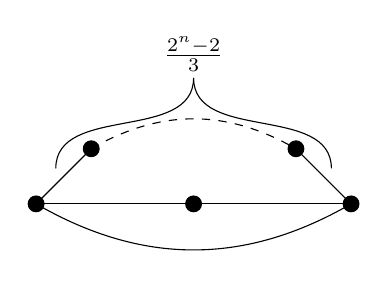
\begin{tikzpicture}

\draw (0,0) to (4,0) ;
\draw (0,0) to [out=-30, in=-150] (4,0) ;
\draw (0,0) to (.7,.7) ;
\draw (3.3,.7) to (4,0) ;
\draw [dashed] (.7,.7) to [out=30, in=150] (3.3,.7) ;

\draw [fill] (0,0) circle [radius=.1] ;
\draw [fill] (4,0) circle [radius=.1] ;
\draw [fill] (2,0) circle [radius=.1] ;
\draw [fill] (.7,.7) circle [radius=.1] ;
\draw [fill] (3.3,.7) circle [radius=.1] ;

\draw (.25,.45) to  [out=90, in=-90] (2,1.6) ;
\draw (3.75,.45) to  [out=90, in=-90] (2,1.6) ;

\node at (2,1.9) {$\frac{2^{n}-2}{3}$} ;

\end{tikzpicture}
\end{center}
    
Case 3b: For $n$ even take $\left\{1,1,1,
  \frac{2^{n}-1}{3}\right\}_{b}$. To check that the divisor $D=v-w$
where $w$ is a trivalent vertex and $v$ is the adjacent vertex on edge
subdivided $\frac{2^{n}-1}{3}$ times has order $2^{n}$, by using the
slope definition of the monodromy pairing by defining the function
such that all slopes are increasing in the direction of $v$ and
decreasing from $w$.  This gives the linear equations
\begin{equation*}
a+b+c+d=2^{t}
\end{equation*}
\begin{equation*}
a=b=c
\end{equation*}
\begin{equation*}
a+\left(\frac{2^{n}-1}{3}-1 \right)(a+b+c)=d
\end{equation*}
where $a$ is the slope on one of the undivided edges
$b$ is the slope on another of the undivided edges,  $c$ is the
slope on the third undivided edge and $d$ is the slope on
the edge between $v$ and $w$.
This results in the equation 
\begin{equation*}
2^na=2^t
\end{equation*}
Since $t$ is at most $n$ and $t=n$ is the only solution such that $a$ has nonnegative  integer value the order of this element must be $2^{n}$. Furthermore $d=2^{n}-3$ implying that the pairing of $D$ with itself is $\frac{2^{n}-3}{2^{n}}$, which isisomorphic to $\CP$ by  \ref{lemma:2-group iso}.

%C pairing n even
\begin{center}
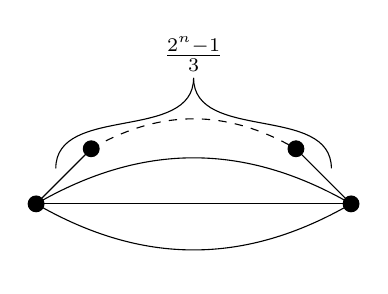
\begin{tikzpicture}

\draw (0,0) to (4,0) ;
\draw (0,0) to [out=-30, in=-150] (4,0) ;
\draw (0,0) to [out=30, in=150] (4,0) ;
\draw (0,0) to (.7,.7) ;
\draw (3.3,.7) to (4,0) ;
\draw [dashed] (.7,.7) to [out=30, in=150] (3.3,.7) ;

\draw [fill] (0,0) circle [radius=.1] ;
\draw [fill] (4,0) circle [radius=.1] ;

\draw [fill] (.7,.7) circle [radius=.1] ;
\draw [fill] (3.3,.7) circle [radius=.1] ;

\draw (.25,.45) to  [out=90, in=-90] (2,1.6) ;
\draw (3.75,.45) to  [out=90, in=-90] (2,1.6) ;

\node at (2,1.9) {$\frac{2^{n}-1}{3}$} ;

\end{tikzpicture}
\end{center}
    
    Case 4a: For odd $n$ take $\left\{1, 2,
\frac{2^{n}-2}{3}\right\}_{c}$. To check that the divisor
$D=v-w$ where $w$ is the vertex with degree has $\frac{2^{n}+4}{3}$ and
$v$ is the vertex with degree has $\frac{2^{n}+1}{3}$ has order
$2^{n}$ one can use the slope definition of the monodromy pairing. Taking the piecewise linear function such that the slopes go away from $w$ and towards $v$ one
obtains the following linear equations,
\begin{equation*}
\frac{2^{n}-2}{3}a+2b=2^{t}
\end{equation*}
\begin{equation*}
a=3b
\end{equation*}
where $a$ is slope on set of $\frac{2^{n}-2}{3}$ edges, and
$b$ is slope on the doubled edges. Since $t$ is at most $n$ and $t=n$ is the only solution such that $b$ has nonnegative integer value the order of this element must be $2^{n}$. This also implies that the pairing of $D$ with itself is $\frac{3}{2^{n}}$, as the equations have solution $a=3$. This pairing is isomorphic to
$\DP$ by  \ref{lemma:2-group iso}.

%D pairing n odd
\begin{center}
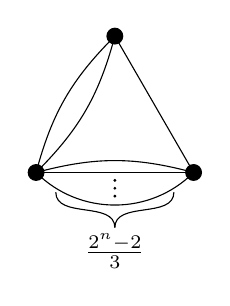
\begin{tikzpicture}

\draw (0:0) [out=45, in=-105] to (60:2) ;
\draw (0:0) [out=75, in=-135] to (60:2) ;
\draw (0:0) [out=15, in=165] to (0:2) ;
\draw (0:0) [out=0, in=180] to (0:2) ;
\draw (0:0) [out=-45, in=-135] to (0:2) ;
\draw (60:2) to (0:2) ;

\draw [fill] (1, -.3) circle [radius=.01] ;
\draw [fill] (1, -.2) circle [radius=.01] ;
\draw [fill] (1, -.1) circle [radius=.01] ;

\draw (.25,-.25) [out=-90, in=90] to (1,-.7) ;
\draw (1.75,-.25) [out=-90, in=90] to (1,-.7) ;

\draw [fill] (0, 0) circle [radius=.1] ;
\draw [fill] (0:2) circle [radius=.1] ;
\draw [fill] (60: 2) circle [radius=.1] ;

\node at (1, -1) {$\frac{2^{n}-2}{3}$} ;

\end{tikzpicture}
\end{center}
    
    Case 4b: For even $n$ take $\left\{1, 1, 1,
\frac{2^{n}-1}{3}\right\}$. To check that the divisor $D=v-w$,
where $w$ is one of the vertices with degree $\frac{2^{n}+2}{3}$
and $v$ is the other vertex with degree $\frac{2^{n}+2}{3}$, has
order $2^{n}$, use the slope definition of the monodromy pairing. Taking the piecewise linear function such that the slopes are increasing towards $w$ and away from $v$, one arrives at the linear equations
\begin{equation*}
b+ \frac{2^{n}-1}{3}a=2^{t}
\end{equation*}
\begin{equation*}
3b=a
\end{equation*}
where $a$ is the slope on edge copied $\frac{2^{n}-1}{3}$ times, and $b$
is slope on the edges that aren't copied. Since $t$ is at most $n$ and $t=n$ is the only solution such that $b$ has nonnegative integer value the order of this element must be $2^{n}$. This also implies that the pairing of $D$ with itself is $\frac{3}{2^{n}}$, as the equations have solution $a=3$. This pairing is isomorphic to
$\DP$ by  \ref{lemma:2-group iso}.

%D pairing n even
\begin{center}
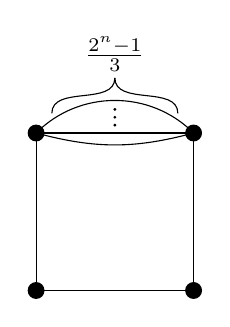
\begin{tikzpicture}

\draw (0,0) to (0,2) ;
\draw (0,0) to (2,0) ;
\draw (2,0) to (2,2) ;
\draw (0,2) to (2,2) ;
\draw (0,2) to [out=-15, in=-165] (2,2) ;
\draw (0,2) to [out=45, in=135] (2,2) ;

\draw [fill] (1, 2.1) circle [radius=.01] ;
\draw [fill] (1, 2.2) circle [radius=.01] ;
\draw [fill] (1, 2.3) circle [radius=.01] ;

\draw (.2,2.25) [out=90, in=-90] to (1,2.7) ;
\draw (1.8,2.25) [out=90, in=-90] to (1,2.7) ;

\node at (1, 3) {$\frac{2^{n}-1}{3}$} ;

\draw [fill] (0,0) circle [radius=.1] ;
\draw [fill] (2,2) circle [radius=.1] ;
\draw [fill] (2,0) circle [radius=.1] ;
\draw [fill] (0,2) circle [radius=.1] ;

\end{tikzpicture}
\end{center}
\end{proof}

%C_{4}
\begin{center}
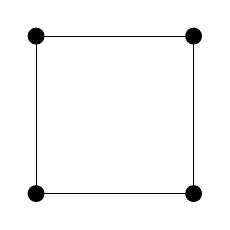
\begin{tikzpicture}

\draw (0,0) to (0,2) ;
\draw (0,0) to (2,0) ;
\draw (2,0) to (2,2) ;
\draw (0,2) to (2,2) ;

\draw [fill] (0,0) circle [radius=.1] ;
\draw [fill] (2,2) circle [radius=.1] ;
\draw [fill] (2,0) circle [radius=.1] ;
\draw [fill] (0,2) circle [radius=.1] ;

\end{tikzpicture}
\end{center}

%B_{4}
\begin{center}
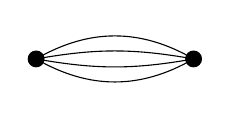
\begin{tikzpicture}

\draw (0,0) to [out=10, in=170] (2,0) ;
\draw (0,0) to [out=-10, in=-170] (2,0) ;
\draw (0,0) to [out=30, in=150] (2,0) ;
\draw (0,0) to [out=-30, in=-150] (2,0) ;

\draw [fill] (0,0) circle [radius=.1] ;
\draw [fill] (2,0) circle [radius=.1] ;

\end{tikzpicture}
\end{center}

\begin{center}
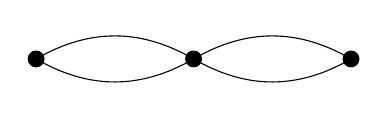
\begin{tikzpicture}

\draw (0,0) to [out=30, in=150] (2,0) ;
\draw (0,0) to [out=-30, in=-150] (2,0) ;
\draw (2,0) to [out=30, in=150] (4,0) ;
\draw (2,0) to [out=-30, in=-150] (4,0) ;

\draw [fill] (0,0) circle [radius=.1] ;
\draw [fill] (2,0) circle [radius=.1] ;
\draw [fill] (4,0) circle [radius=.1] ;

\end{tikzpicture}
\end{center}

Each of the above constructions gives a graph with cyclic Jacobian,
giving four of the six generators for 2-groups with pairing. We have
few concrete results relating to the remaining two
generators. However, we may still make the following observation:

\begin{thm}
  For any $k \ge 1$, there is no graph $G$ such that $\Jac(G) \simeq
  (\mathcal{E}_2)^k$. 
\end{thm}
\begin{proof}
  This is a result of the characterization of graphs $G$ with $\Jac(G)
  \simeq (\Z/2\Z)^k$, given in Section 1. We see that any such graph
  has Jacobian isomorphic to $(\AP)^k$.
\end{proof}

This result, combined with our inability to construct \emph{any} graph
$G$ that yields the group $\EP$, leads us to make the following:

\begin{conj}
  There is no graph $G$ such that $\Jac(G) \simeq \EP$.
\end{conj}

We note, however, that there do exist examples of graphs $G$ such that
for some subgroup $H \subset \Jac(G)$, if $\pair{\cdot}{\cdot}\big|_H$ is
the monodromy pairing on $\Jac(G)$ restricted to $H$, then $(H,
\pair{\cdot}{\cdot}\big|_H) \simeq \EP$. In particular, take $G$ to be
the following graph:

[PICTURE GOES HERE, ONCE WE ACTUALLY FIGURE OUT WHAT THIS GRAPH SHOULD
BE]

We have even fewer results regarding $\FP$. We note that the complete
graph $K_4$ is an example of a graph with Jacobian isomorphic to
$\mathcal{F}_4$, but we were unable to find other examples of graphs
that provide this pairing.

\subsection{Simple graphs}
As in Section 1, some of the constructions given above are only
possible if we allow multiple edges on our graphs. We do not have a
broad result concerning groups with pairing that \emph{can} arise as
Jacobians of multigraphs that \emph{cannot} arise as Jacobians of
simple graphs. However, we observe that such groups do in fact exist:

\begin{thm}
  Let $\Gamma_\mathfrak{r} \simeq (\Z/3\Z, \mathfrak{r})$, and
  $\Gamma_\mathfrak{n} \simeq (\Z/3\Z, \mathfrak{n})$. For any odd
  integer $k$, there is no simple graph $G$ such that
  \begin{align*}
      \Jac(G) \simeq (\Gamma_\mathfrak{r})^k, \text{ or } \\
      \Jac(G) \simeq (\Gamma_\mathfrak{r})^k \times \Gamma_\mathfrak{n}
  \end{align*}
\end{thm}
\begin{proof}
Lemma \ref{lem:delta_le_mu} shows that the only biconnected simple
graph with Jacobian of the form $(\Z/3\Z)^k$ is the $3$-cycle
$C_3$. The monodromy pairing on $\Jac(C_3)$ is the nonresidue pairing
$\mathfrak{n}$, and the groups with pairing given above do not arise
as powers of $\Z/3\Z$ with this pairing. 
\end{proof}

\end{document}